% Charlotte Geiger - Manuel Lippert - Leonard Schatt
% Physikalisches Praktikum

% Teilaufgabe X

\section{Faltung zweier Rechtecksfunktionen}

Um eine Faltung zu berechnen gibt es mehrere Möglichkeiten. Ein Lösung ist es den Faltungsatz zu verwenden. Dieser besagt, dass bei Funktionen $f$ und $g$ im Ortsraum mit den 
zugehörigen Funktionen $\tilde{f}$ und $\tilde{g}$ im Fourierraum gilt:
\begin{equation}  \label{faltungssatz}
    f\ast g = \mathfrak{F}^{-1}(\tilde{f} \cdot \tilde{g}  ) = g \ast f
\end{equation}\\
Dieses Vorgehen ist aber manchmal etwas umständlich. In einfacheren Fällen wie diesem hier ist eine graphischen Lösung einfacher. 
Bei dieser Zeichet man die Graphen beider Funktionen. Dann spiegelt man den zu verknüfenden Graphen an der y-Achse und "schiebt" diesen dann über den ersten Graphen. 
Die Fläche die sie sich überschneiden ist dann die Funktion $f \ast g $.\\
In diesem Fall nehmen wir zwei Rechtecksfuntionen mit Höhe eins und Breite $a$ bei Rechteck 1 und $b$ bei Rechteck 2. Die beiden Rechtecke sind Achsensymetrisch bezüglisch der y-Achse.
\begin{figure}[htb]
    \centering
        \begin{minipage}[t]{0.45\linewidth}
            \centering
            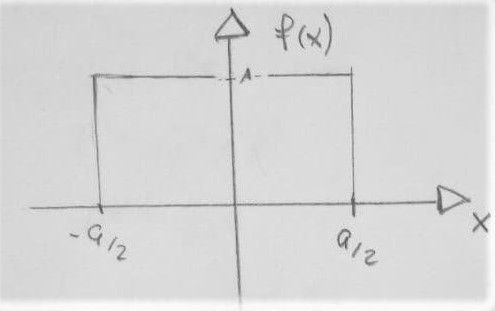
\includegraphics[width=4cm]{Bilder/FzV/frage6_1.jpg}
            \caption{Skizze von $f$}
        \end{minipage}
        \hfill
        \begin{minipage}[t]{0.45\linewidth}
            \centering
            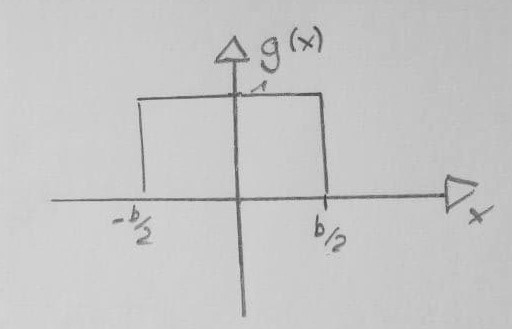
\includegraphics[width=4cm]{Bilder/FzV/frage6_2.jpg}
            \caption{Skizze von $g$}
        \end{minipage}
   
    
    %\label{fig:meine-grafik}
\end{figure}
Jetzt können zwei Fälle Auftreten:\\
 \begin{itemize}
    \item Fall 1: $a=b$
 
            In diesem Fall entsteht ein perfektes Dreieck, da nur in einem Punkt die volle Fläche erreicht ist.
            \begin{figure}[h]
                \centering
                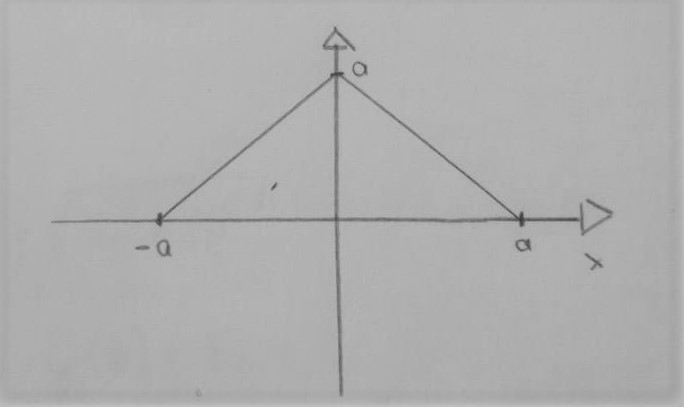
\includegraphics[width = 4cm]{Bilder/FzV/frage6_3.jpg}
                \caption{Skizze von $f \ast g$ mit $a=b$}
                \label{faltung}
            \end{figure}
        Die maximale Überschneidung der beiden Graphen ist daher $a \cdot 1 = a$.
    \item Fall 2: $a'  > b'$
        Diesmal sind die beiden Dreieck nicht Deckungsgleich. Deshalb ist die maximale Überschneidung hier nur $b' \cdot 1 = b'$. 
        Es ist also kein Dreieck wie in Abbildung \ref{faltung}, sondern dem Dreieck wurde seine Spitze abgeschnitten. 
        \newpage
        \begin{figure}[h]
            \centering
            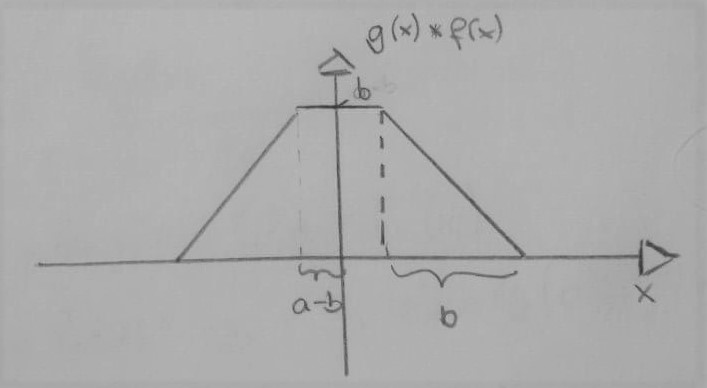
\includegraphics[width = 4cm]{Bilder/FzV/frage6_4.jpg}
            \caption{Skizze von $f\ast g$ mit $b < a$}
        \end{figure}
    \item Fall 3: $a''< b''$
        Dieser Fall ist identsich zu Fall zwei, da man O.b.d.A. $a''$ und $b''$ vertauschen kann laut Gleichung \ref{faltungssatz}.
        Das heißt, in diesem Fall erhält man wieder ein angeflachtes Dreieck.
   \end{itemize}
An dieser Stell sieht man, dass es sinvoll ist die Eingangs- und Ausgangsspaltbreite gleich zu wählen, da man dann den größten "Peak" bekommt. 
Wenn man sie nicht gleichgroß wählt schneidet es einem den höchsten Ausschlag ab, was schlecht für die Messung ist. Man sollte jedoch die Spalte nicht zu klein machen, da dann die Intensität nach den Spalten nachlässt. 

